\section{Ejemplos}

\subsection{Método de Grimmett (2004) - \textit{Systematic rounding}}

Se podría decir que este método es el más "natural" que a uno se le ocurriría a la hora de diseñar
un sistema aleatorizado \textit{quota-compliant}, propuesto por \cita{Grimmett01042004}:
reordenando los partidos de forma aleatoria, se le asigna a cada partido un intervalo de longitud igual a 
su resto $p_i$ (con $p_i$ el resto del partido $i$ luego del reordenamiento), colocando los intervalos uno a 
continuación del otro en el intervalo $[0,k]$, que, 
como $p \in \Omega_n^{k}$, resulta completamente cubierto por los intervalitos. Llamamos $s_i = \sum_{j=1}^{i}p_i$.

\begin{figure}[h!]
\centering
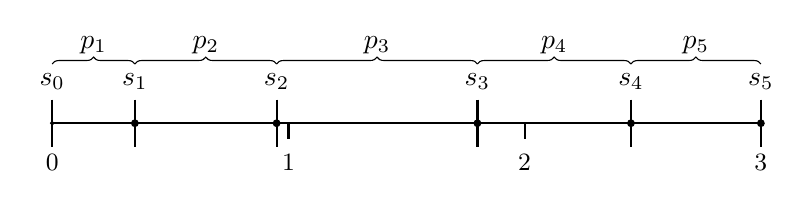
\begin{tikzpicture}[x=3cm, y=1cm] % escala horizontal: 3cm por unidad (0..3 ocuparán 9cm)
    % --- Posiciones (ajustá estos valores "aleatorios" si querés) ---
    \def\sone{0.35}
    \def\stwo{0.95}
    \def\sthree{1.80}
    \def\sfour{2.45}
    \def\sfive{3}

    % --- Eje principal ---
    \draw[thick] (0,0) -- (3,0);

    % --- Marcas enteras 0..3 ---
    \foreach \x in {0,1,2,3} {
        \draw[thick] (\x,0) -- (\x,-0.2) node[below=2pt] {\small $\x$};
    }

    % --- Marcas largas para s_i ---
    \draw[thick] (0.0,0.3) -- (0.0,-0.30) node[above=17pt] {$s_0$};
    \draw[thick] (\sone,0.3) -- (\sone,-0.30) node[above=17pt] {$s_1$};
    \draw[thick] (\stwo,0.3) -- (\stwo,-0.30) node[above=17pt] {$s_2$};
    \draw[thick] (\sthree,0.3) -- (\sthree,-0.30) node[above=17pt] {$s_3$};
    \draw[thick] (\sfour,0.3) -- (\sfour,-0.30) node[above=17pt] {$s_4$};
    \draw[thick] (\sfive,0.3) -- (\sfive,-0.30) node[above=17pt] {$s_5$};

    % --- Puntos visibles (opcional) ---
    \filldraw (0,0) circle (0.6pt) node[above left=2pt] {};
    \filldraw (\sone,0) circle (1.2pt) node[above=5pt] {};
    \filldraw (\stwo,0) circle (1.2pt) node[above=5pt] {};
    \filldraw (\sthree,0) circle (1.2pt) node[above=5pt] {};
    \filldraw (\sfour,0) circle (1.2pt) node[above=5pt] {};
    \filldraw (\sfive,0) circle (1.2pt) node[above=5pt] {};

    % --- Segmentos p_i como corchetes/braces encima del eje ---
    % (0 -> s1) = p1
    \draw[decoration={brace,raise=18pt},decorate]
        (0,0.12) -- (\sone,0.12) node[midway,above=18pt] {$p_1$};

    % (s1 -> s2) = p2
    \draw[decoration={brace,raise=18pt},decorate]
        (\sone,0.12) -- (\stwo,0.12) node[midway,above=18pt] {$p_2$};

    % (s2 -> s3) = p3
    \draw[decoration={brace,raise=18pt},decorate]
        (\stwo,0.12) -- (\sthree,0.12) node[midway,above=18pt] {$p_3$};

    % (s3 -> s4) = p4
    \draw[decoration={brace,raise=18pt},decorate]
        (\sthree,0.12) -- (\sfour,0.12) node[midway,above=18pt] {$p_4$};
    
    % (s4 -> s5) = p5
    \draw[decoration={brace,raise=18pt},decorate]
        (\sfour,0.12) -- (\sfive,0.12) node[midway,above=18pt] {$p_5$};

\end{tikzpicture}
\caption{Segmento ilustrativo de la disposición inicial del método de Grimmett, con $n=5$ y $k=3$. La longitud de los segmentos $[s_{i-1}, s_i]$ es $p_i$ para $i \in \{1, \dots, 5 \}$.
Los puntos $s_i$ están ubicados en las posiciones $s_i = \sum_{j=1}^{i}p_i$.}
\label{fig:grimmett_1}
\end{figure}


Posteriormente, se sortea una variable $U \sim \textit{Unif}\ [0,1)$, y se desplazan los puntos $s_i$ a $s'_i = s_i + U$.
Los intervalos $[s'_{i-1}, s'_i)$ son iguales a los originales desplazados en $U$, por lo que siguen midiendo $p_i$, 
y la probabilidad de que contengan un entero es proporcional a $p_i$.
De esta forma, asignando las bancas a los partidos cuyos intervalos contengan un entero se tiene una asignación de las $k$ bancas pendientes
de ser repartidas, puesto que en el intervalo $[U, k + U)$ hay exactamente $k$ enteros.

\begin{figure}[h!]
    \centering
    \begin{tikzpicture}[x=3cm, y=1cm] % escala horizontal: 3cm por unidad (0..3 ocuparán 9cm)
        % --- Posiciones (ajustá estos valores "aleatorios" si querés) ---
        \def\unif{0.23}
        \def\szero{\unif}
        \def\sone{0.35 + \unif}
        \def\stwo{0.95 + \unif}
        \def\sthree{1.80 + \unif}
        \def\sfour{2.45 + \unif}
        \def\sfive{3 + \unif}
    
        % --- Eje principal ---
        \draw[thick] (0,0) -- (\sfive,0);
    
        % --- Marcas enteras 0..3 ---
        \foreach \x in {0,1,2,3} {
            \draw[thick] (\x,0) -- (\x,-0.2) node[below=2pt] {\small $\x$};
        }
    
        % --- Marcas largas para s_i ---
        \draw[thick] (\szero,0.3) -- (\szero,-0.30) node[above=14pt] {$U = s'_0$};
        \draw[thick] (\sone,0.3) -- (\sone,-0.30) node[above=14pt] {$s'_1$};
        \draw[thick] (\stwo,0.3) -- (\stwo,-0.30) node[above=14pt] {$s'_2$};
        \draw[thick] (\sthree,0.3) -- (\sthree,-0.30) node[above=14pt] {$s'_3$};
        \draw[thick] (\sfour,0.3) -- (\sfour,-0.30) node[above=14pt] {$s'_4$};
        \draw[thick] (\sfive,0.3) -- (\sfive,-0.30) node[above=14pt] {$s'_5$};
    
        % --- Puntos visibles (opcional) ---
        \filldraw (0,0) circle (0.6pt) node[above left=2pt] {};
        \filldraw (\szero,0) circle (1.2pt) node[above=5pt] {};
        \filldraw (\sone,0) circle (1.2pt) node[above=5pt] {};
        \filldraw (\stwo,0) circle (1.2pt) node[above=5pt] {};
        \filldraw (\sthree,0) circle (1.2pt) node[above=5pt] {};
        \filldraw (\sfour,0) circle (1.2pt) node[above=5pt] {};
        \filldraw (\sfive,0) circle (1.2pt) node[above=5pt] {};
    
        % --- Segmentos p_i como corchetes/braces encima del eje ---
        % (0 -> s1) = p1
        \draw[decoration={brace,raise=18pt},decorate]
            (\szero,0.12) -- (\sone,0.12) node[midway,above=18pt] {$p_1$};
    
        % (s1 -> s2) = p2
        \draw[decoration={brace,raise=18pt}, draw = rojoOscuro, decorate, line width=0.3mm]
            (\sone,0.12) -- (\stwo,0.12) node[midway,above=18pt, rojoOscuro] {$p_2$};
    
        % (s2 -> s3) = p3
        \draw[decoration={brace,raise=18pt}, draw = rojoOscuro, decorate, line width=0.3mm]
            (\stwo,0.12) -- (\sthree,0.12) node[midway,above=18pt, rojoOscuro] {$p_3$};
    
        % (s3 -> s4) = p4
        \draw[decoration={brace,raise=18pt},decorate]
            (\sthree,0.12) -- (\sfour,0.12) node[midway,above=18pt] {$p_4$};
        
        % (s4 -> s5) = p5
        \draw[decoration={brace,raise=18pt}, draw = rojoOscuro, decorate, line width=0.3mm]
            (\sfour,0.12) -- (\sfive,0.12) node[midway,above=18pt, rojoOscuro] {$p_5$};
    
    \end{tikzpicture}
    \caption{Segmento ilustrativo de la disposición final del ejemplo anterior. Los segmentos $[s'_{i-1}, s'_i]$ fueron desplazados en $U$.
    Marcados en \textcolor{rojoOscuro}{rojo} se encuentran los segmentos que contienen a un entero, correspondientes a los
    partidos 2, 3 y 5.}
    \label{fig:grimmett2}
\end{figure}

% ------------------------------------------------------
\subsection{Formulación como problema de optimización de medida}

Pensando en que estamos buscando algoritmos aleatorizados que seleccionen conjuntos de $k$ 
partidos verificando cumplir con las probabilidades marginales dadas por $p_i$, 
podemos pensar en que estamos buscando distribuciones de probabilidad sobre un espacio muestral dado 
por los conjuntos $S \in \binom{[n]}{k}$. 
Si además buscamos que dicha distribución sea un punto extremal de algún funcional $g$ sobre el 
espacio de medidas definidas en $\binom{[n]}{k}$, se abre la posibilidad de construir un método 
de distribución de bancas a partir de buscar las probabilidades de selección de cada conjunto 
encontrando una solución factible del siguiente problema:

Encontrar $\mu:\binom{[n]}{k} \rightarrow \mathbb{R}_{\geq 0}$ solución de 

\[
\begin{aligned}
\max\limits_{\mu} g(\mu)\ & & \\
\text{s.a.}\
\left\{
\begin{aligned}
\sum_{B \in \binom{[n]}{k}}{\mu(B)} = 1 & &\\
\sum_{\substack{B \in \binom{[n]}{k} \\ B \ \ni \ i}}{\mu(B)} = p_i & \quad \forall i \in [n] &
\end{aligned}
\right.
\end{aligned}
\]

\vspace{0.5cm}

A partir de este planteo, surge la siguiente serie de preguntas:
\vspace{0.25cm}

\begin{itemize}
    \item ¿Qué $g$ se puede elegir para que la medida inducida por el algoritmo de \textit{Sampford} 
    sea la solución óptima? Sabemos que dicha medida es factible.
    \item Más en general, ¿qué $g$ se puede elegir para encontrar una medida que verifique \textit{monotonía de selección}?
    \item ¿existe algún modo de enunciar la propiedad de \textit{monotonía de selección} a partir de 
    $\mu_A$, $p_i$ y $p'_i$ de forma lineal como para introducirla en forma de restricción?
    \item ¿Tendría sentido que el funcional $g$ busque minimizar la distancia con respecto a la 
    medida inducida por el algoritmo de \textit{Sampford}?
\end{itemize}

\vspace{0.5cm}

Vale observar que la primera restricción es innecesaria, pues si sumamos la segunda restricción 
sobre $i \in [n]$,

\begin{align*}
    \sum_{i=1}^{n}\sum_{\substack{B \in \binom{[n]}{k} \\ B \ \ni \ i}}{\mu(B)} &= \sum_{i=1}^{n} p_i \\
    k \sum_{\substack{B \in \binom{[n]}{k}}}{\mu(B)} &= k , \\
\end{align*}

pues del lado izquierdo estamos contando $k$ veces cada conjunto 
(1 vez por cada elemento que contiene, es decir, $k$ veces en total), 
y del lado derecho nos queda la suma de los $p_i$ que es exactamente $k$. 

Dividiendo por $k$ a ambos lados, se tiene la primera restricción:

$$\sum_{B \in \binom{[n]}{k}}{\mu(B)} = 1$$

Es importante ver que, más allá de cuál sea la función objetivo $g$, existe 
una única solución para los casos en los que $k \in \{ 1, n-1 \}$, pues en ambos casos 
el sistema resultante de las restricciones es lineal de $n \times n$ y de rango $n$. En consecuencia, 
hay solamente una solución factible, dada por $\mathbb{P}_p(S = \{ i \}) = p_i$ en el caso de $k=1$, 
o por $\mathbb{P}_p(S = [n] \setminus \{ i \}) = 1 - p_i$ en el caso de $k=n-1$. Además, para estos dos
valores de $k \in \{ 1, n-1 \}$, la linealidad sobre los $p_i$ provoca que cualquier método verifique
\textit{monotonía de selección}.

Por otro lado, incorporación de la restricción provoca que automáticamente se verifique \textit{proporcionalidad
Ex-Ante} para cualquier solución de este problema, por lo que el interés sobre métodos fabricados 
a partir de esta formulación radicará en verificar si cumplen \textit{monotonía de selección} para $k \notin \{ 1, n-1 \}$.

% ------------------------------------------------------
\subsection{Conditional Poisson Rounding - Máxima Entropía}

Propuesto como método de $\pi ps$ por \cita{10.1093/biomet/81.3.457} y retomado 
como método de \textit{apportionment} en \cita{correa2024monotonerandomizedapportionment}, 
este método consiste en hacer exactamente el planteo de la sección anterior, utilizando como
función objetivo la entropía de la distribución, dada por 

$$H(S) = \sum_{B \in \binom{[n]}{k}}{\mu(B) \frac{1}{\log(\mu(B))}}$$

donde $S \in \binom{[n]}{k}$ tiene distribución dada por $\mu$.

A la hora de pensar en la motivación de este método surge la duda de por qué se busca maximizar
la entropía. Considerando que la entropía cuantifica la cantidad de información o incertidumbre 
a priori que se tiene sobre los resultados posibles al samplear de una distribución, en cierta 
forma se está buscando tener "la menor cantidad información a priori" sobre qué subconjunto de $k$ 
partidos será seleccionado. En otras palabras, es un modo de intentar maximizar la incertidumbre previa que se tiene
acerca de qué partidos serán seleccionados, siempre sujetos a la restricción de las probabilidades
condicionales.

\cita{singh2013entropyoptimizationcounting} y \cita{10.1093/biomet/81.3.457} caracterizan a esta distribución como una distribución
producto: la solución del problema verifica que 
$$\mu(S) = \prod_{i \in S}{\lambda_i},$$ 
con $\vec{\lambda} \in \mathbb{R}_{>0}^n$ obtenido mediante la formulación dual del problema.

Otra forma en la que \cita{10.1093/biomet/81.3.457} caracteriza a esta distribución es la que le da el nombre 
de \textit{Conditional Poisson Rounding}: se definen variables $Z_i \sim \textit{Bernoulli}(p_i)$ 
independientes (Poisson Trial), y la distribución del vector $X = (X_1, \dots, X_n)$ como 
la distribución del vector $Z$ condicional a que $\sum_{i=1}^{n}{Z_i} = k$. De esta forma, 
se construye el conjunto de partidos seleccionados a partir de un \textit{Poisson Trial} condicionado
a tener exactamente $k$ elementos.

Las 3 formas equivalentes de definir este método brindan un sistema \textit{quota-compliant} y
\textit{proporcional ex-ante}:
por construcción resulta automáticamente \textit{quota-compliant}, y la restricción de las probabilidades
marginales en la formulación de máxima entropía lo hace \textit{proporcional ex-ante}. Cabe preguntarse 
¿verificará también \textit{monotonía de selección}?
Lo veremos en la próxima sección.

Una cuestión importante relativa a este método es el hecho de que depende fuertemente de ser computado mediante 
algún solver de optimización, dado que no hay forma analítica de encontrar la distribución de máxima entropía. 
Si bien en \cita{correa2024monotonerandomizedapportionment}, citando a \cita{Tillé2025}, proponen encontrar el vector 
$\vec{\lambda}$ utilizando el método de Newton, esta solución tampoco resulta exacta.
Esto provoca que siempre exista un grado de imprecisión en la distribución encontrada, propia del error numérico
de los solvers computacionales y los métodos numéricos como Newton.

% ------------------------------------------------------
\subsection{Algoritmo de Sampford (67')}

Introducimos el algoritmo de \textit{rounding} introducido por Sampford \cita{10.1093/biomet/54.3-4.499}. 
En la siguiente sección analizaremos las propiedades que cumple, siguiendo el trabajo de \cita{correa2024monotonerandomizedapportionment}.

\vspace{1em}

\begin{algorithm}[H]
\SetAlgoLined
\KwResult{Encontrar un conjunto aleatorio de K partidos de acuerdo a las probabilidades marginales dadas por $p_i$, con reposición}
 Inicializamos $S = \{ \} $ \;
 Samplear un elemento con probabilidad proporcional a $p_i$ y asignarle una banca agregándolo a S\;
 Reponer el elemento\;
 \For{$1 \leq j \leq K-1$}{
  Samplear un elemento con probabilidad proporcional a $\frac{p_i}{1-p_i}$ y agregarlo a S\;
  Reponer\;
 }
 \If{$|S| = K$}
 {\Return S\;}
 \Else{Reiniciar todo el procedimiento \;}
 \caption{Sampford}
\end{algorithm}

\vspace{1em}

La intuición de definir las probabilidades de los sampleos $2, \dots, k$ proporcionales a $\frac{p_i}{1-p_i}$ no
es para nada clara. No obstante, veremos que al ser sampleo sin reposición, la utilización de estas probabilidades resulta en
que el método sea \textit{proporcional ex-ante}. Una desventaja de este método es que no tiene una cota estricta en la cantidad de
iteraciones que realiza, puesto que en cada ejecución hay probabilidad positiva de seleccionar 2 veces un mismo elemento, ocasionando
que se deba reiniciar el procedimiento.

Como bien observan en \cita{correa2024monotonerandomizedapportionment}, la rareza -- o el ingenio -- de este método radica en la
elección de las probabilidades de sampleo: si los $k$ elementos fueran elegidos con probabilidades proporcionales a $\frac{p_1}{1-p_i}$, se tendría
una distribución producto en la que la probabilidad de seleccionar a un conjunto $A$ sería proporcional a $\prod_{i \in A}{\frac{p_1}{1-p_i}}$.
Por el resultado de \cita{singh2013entropyoptimizationcounting}, esta distribución producto correspondería a una distribución de 
máxima entropía, pero con probabilidades marginales erróneas. Lo extraño es que, sabiendo que no hay forma analítica de encontrar una
fórmula cerrada para deducir las probabilidades de \textit{Conditional Poisson Rounding}, simplemente corrigiendo las probabilidades 
de selección del primer elemento por $p_i$ en lugar de $\frac{p_i}{1-p_i}$, se consigue que las probabilidades marginales sean las 
deseadas (y por ende, que el método sea \textit{proporcional ex-ante}, como demostraremos en la próxima sección).

% ------------------------------------------------------
\subsection{Algoritmo de Brewer (63')}

Propuesto en \cita{brewer_sampling}, este algoritmo tampoco goza de demasiada transparencia a la hora de entender
la forma en la que se redefinen iterativamente las probabilidades de sampleo. 

\begin{algorithm}[H]
\SetAlgoLined
\KwResult{Encontrar un conjunto aleatorio de K partidos de acuerdo a las probabilidades marginales dadas por $p_i$, sin reposición}
 Inicializamos $S = \{ \} $, $N = \{ 1, \dots, n\} $\;
 \For{$t = k, \dots, 1$}{
 Definir $q_i = \frac{p_i}{\sum\limits_{j \in N}{p_j}} \quad \forall i \in N$ \;
 Seleccionar $i$ con probabilidad proporcional a $\frac{q_i (1- q_i)}{1-t q_i}$ \;
 $N = N \setminus \{ i \}$ \;
 }
 \Return S \;
 \caption{Brewer}
\end{algorithm}

Introducimos este último algoritmo por el hecho de que fue objeto de estudio durante la presente tesis:
nos interesará conocer si verifica \textit{monotonía de selección}.

